\documentclass[10pt,a4paper]{article}
\usepackage[utf8]{inputenc}
\usepackage[english]{babel}
\usepackage{amsmath}
\usepackage{amsfonts}
\usepackage{amssymb}
\usepackage{graphicx}
\author{Karl Johan Andreasson \and Josef Sunesson}
\title{Green Elevator}
\begin{document}
\maketitle

\begin{abstract} 
This report handles the implementation of the Green Elevator project in the course Concurrent Programming. The developed controller handles OK.
\end{abstract}

\section{Introduction}
\label{sec:intro}
Elevators are present in almost every apartment complex with more than 1 floor. The controller for these elevators has to receive information about the button presses the users make and schedule the elevators accordingly.

To implement this controller to handle the button presses and also the position updates coming from the elevator is the goal of the project. There are several different aspects that has to be considered when scheduling the different elevator cabins. The most important aspects are to minimize waiting time before a cabin comes to serve the user and to minimize the time spent traveling to the desired floor. Another aspect to take into consideration when implementing a scheduling algorithm for the elevator cabins are power consumption.

In the elevator scheduling problem there are hard deadlines to meet once a press of a button has been made. These deadlines are both to not end up with frustrated end users because the controller of the elevators are too slow to schedule the elevators and to not cause the elevators to miss stopping at a floor because the scheduling algorithm was hard at work scheduling another press of a button from a user. To alleviate these problems and to make the solution future proof if the controller should be used with more powerful hardware, a parallelized implementation is desirable.

Another very important aspect of the elevator controller is that it has to provide a fair scheduling of the jobs it receives. No starvation of a job is allowed. Starvation could happen if a job gets postponed because there are other jobs that get scheduled to be executed before and if these jobs continue to arrive the original job is suffering from starvation.

\section{Program outline}
The implementation of the controller of the elevators was made in the language C++ using monitors with locks from the Pthread library for synchronization. C++ was chosen over Java because of the speed increase C++ produces and because both authors prefer to do programming in C++ over Java.

The implementation of the elevator controller uses several threads running simultaneously to minimize the response time of the controller. The threads running are one for every elevator cabin present, one thread that is reading the commands that are coming to the elevators and then dispatching them to either the scheduler or the thread handling the concerned elevator and one last thread to perform scheduling of the jobs.

The threads communicate through monitors and it is also through monitors that synchronization is achieved. The choice of monitors was made because of the abstraction it provides. In the implementation there are several monitors present. One monitor for handling jobs that are to be scheduled, one monitor to handle the communication between the hardware elevator controller and the elevators and one for each elevator cabin. The need of a monitor for communication between the hardware elevator controller and the elevators is because of the choice of implementing the controller of the elevators in C++, the communication is performed over TCP to the hardware elevator controller. This forces the communication to be performed serialized and this is performed using a monitor.

\begin{figure}[!h]
\centering
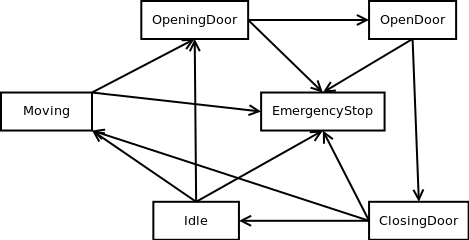
\includegraphics[scale=0.5]{state_transition.png}
\caption{State transitions of an elevator.}
\label{fig:states}
\end{figure}

An elevator is considered as a state machine in the implementation. The states an elevator can have is Idle, Moving, OpeningDoor, ClosingDoor, OpenDoor and EmergencyStop. The state transitions can be found in figure \ref{fig:states}. When considering the elevators as state machines, the scheduling and how elevators handle commands given to them are simplified.

A command in the implementation is a button press either inside one of the elevators or on a floor. The command will be read by the reading thread and passed on to the appropriate vector. This vector is either a vector for elevator specific commands for a specific elevator or a vector inside the scheduling monitor for unscheduled commands.

Every handler for the elevators will loop through a while loop until it is signaled by the main thread that the execution is over. Inside the loop it will check for commands to handle inside the elevator specific command vector. These commands are handled inside the monitor associated with the elevator to provide mutual exclusion. Once the commands are handled the elevator invokes a function called run\_elevator inside the elevator monitor, this function will start the elevator if its idle and close the doors if they are open and the timer controlling how long the door has been open has run out.

% Once a command is received by an elevator monitor it will try to fit it in its vector of floors it is scheduled to stop at. If it is unable to stop at the floor in the command given the monitor will queue it in the unfitted commands vector in the commands to schedule monitor if it was a floor button and discard the command if it came from inside the elevator cabin. If the command was valid it will try to enter it to the vector of scheduled floors. After it was entered into the vector, the vector is sorted either in ascending order for when the elevator is going upwards or descending order if the elevator is going downwards.

\section{Scheduling}
\label{sec:scheduling}

The scheduler is only concerned with scheduling new requests from users coming to the elevator and pressing either up or down depending on the direction they want to go.

What the scheduler does when it gets such a request is to loop over all the elevators. For each elevator, the scheduler asks what the elevators absolute position relative to the request is. If an elevator cannot handle the request, e.g. when an elevator is going upwards and the new request is to go down, the elevator returns a negative value as its absolute position and thereby indicating that it is not available for the scheduler to use.

In the case the elevator does not return a negative value, the scheduler stores the returned value and the elevator that returned that value. When the scheduler has asked all elevators for its absolute position relative the floor of the request, the elevators are sorted according to which was the closest to the floor of the request. Then the scheduler takes the closest elevator and tries to schedule the request to that elevator. This involves asking the elevator for its absolute position
again to assure that the elevator is still able to handle the request in case that elevator has moved since the scheduler asked it the first time. If the elevator cannot handle the request any longer, the next possible elevator is tried and so forth.

If no elevator is able to handle the request to begin with, or if that is the case after checking all the elevators again, the request is added to a FIFO queue of commands that has not been scheduled that the elevators takes requests from regularly. The elevators also make sure to take the first request in the queue in case the elevator turn idle in order to guarantee that every request will eventually be handled.

\section{Handling commands}
\label{sec:commands}
Each elevator has two functions for handling new commands, one for handling position update commands and one for handling button presses either inside or outside the elevator.

The function for handling position updates is the function where the elevator detects if it has reached a new floor. If that floor was the target floor of the elevator, the elevator is stopped and the doors are opened. This function is also responsible keeping track of how the opening and closing of the doors is progressing.

The function for handling button presses is the function that is responsible for ordering the target floors of the elevator when it receives a new button press so that the elevator will go to each target floor in an appropriate order according the direction the elevator has to go in order to serve the target floors it have. Mainly this means that the elevator e.g. will ignore button presses to go down to a floor below its current position in case the elevator is moving upwards.

When the elevator is handling a new button press, it also tries to get requests that have not been possible to schedule to any elevator yet so that no request will be ignored forever.

\section{Evaluation}
\label{sec:eval}
The implementation of the controller for the elevators are evaluated on mainly four different aspects. These aspects are time travelling inside the elevator, time waiting for the elevator, if it is fair or not and finally power consumption.

These aspects has to be weighted against each other because there is no way of achieving a perfect solution in every aspect. An example of this is when there are one person wanting to go from floor two to floor 4 and one person wanting to go from floor three to five. To minimize traveling time for both persons they would have to be handled separately, this would make the time waiting for an elevator to arrive significantly longer if there are only one available elevator. This means that there are no optimal solution to the scheduling problem without weighting the different measuring aspects.

The solution should always be fair regardless of the weighting used. A fair solution does not allow for starvation to happen. There is no way of starvation in the implementation in this project. This is because every command will be handled. Once an elevator cabin reaches an end point in the scheduled direction the elevator monitor will try to schedule an unfitted command before going idle and accepting new commands.

The implementation in this project tries to minimize the time traveling, the time waiting for an elevator as well as power consumption by always checking the nearest valid cabin by the algorithm described in section \ref{sec:scheduling}. This implementation does not perform the optimal way in aspect but provide a fair trade-off.

\section{Conclusion}
\label{sec:conclusion}
\end{document}
